\section{计算模型与几何引擎}
\subsection{引言}

\tkzNamePack{tkz-elements} 宏包不仅仅是一组几何作图命令的集合。它实现了一个基于统一数学模型的、连贯的计算几何引擎。

本章介绍宏包背后的数学与计算基础。虽然大多数用户面对的是 \tkzClass{point}、\tkzClass{line}、\tkzClass{circle}、\tkzClass{triangle} 或 \tkzClass{conic} 这样的高层几何对象，但所有作图最终都依赖于一个紧凑的代数内核和一套精心设计的数值策略。

本章的目的有三：

\begin{itemize}
\item 描述内部使用的数学模型，
\item 说明数值稳健性策略，
\item 阐明支配本引擎的架构原则。
\end{itemize}

本章可以独立阅读，作为对几何引擎的一份技术概览。

\subsection{复平面模型}

平面上的所有点在内部都表示为复数：

\[
z = x + iy,
\]

其中 \(x\) 和 \(y\) 是实坐标。

这一选择为几何计算提供了一个紧凑且代数上自洽的框架。向量的加法、减法、旋转和位似都成为自然的代数运算。

因此，\tkzClass{point} 类具有双重含义：它既是欧几里得平面中的一个几何点，又是代数模型中的一个复数。这种设计避免了分别维护向量抽象和复数抽象，为几何计算提供了一个紧凑、连贯的框架。

复平面表示使我们能够：

\begin{itemize}
\item 直接实现向量运算，
\item 用简洁的式子表达旋转和对称，
\item 通过复数乘法自然地编码方向，
\item 简化行列式和点积的计算。
\end{itemize}

使用复数既保证了优雅，又保证了计算效率。

%--------------------------------------------------------------------
\subsubsection{作为复数的点类}
\label{sub:complex_numbers}

例如，
\begin{verbatim}
z.A = point(1, 2)
z.B = point(1, -1)
\end{verbatim}
定义了两个点对象，它们对应的附标为
\[
z_A = 1 + 2i,
\qquad
z_B = 1 - i.
\]
记号 \verb|z.A| 指存放在表 \verb|z| 中的一个 Lua 对象，
而 \(z_A\) 表示它所对应的复数。

\medskip
如果更愿意使用独立变量（不使用保留表），也可以写成：
\begin{verbatim}
za = point(1, 2)
zb = point(1, -1)
\end{verbatim}
唯一的区别是组织方式：\verb|z.A| 存放在表 \verb|z| 中，而 \verb|za| 是一个普通的 Lua 变量。

\medskip
代数结构通过 Lua 元方法和一小类方法来实现，使标准运算符能够以自然的方式执行几何运算。

%--------------------------------------------------------------------
% 元方法表
%--------------------------------------------------------------------
\begin{center}
  \bgroup
  \catcode`_=12
  \small
  \begin{minipage}{\textwidth}
  \captionof{table}{点（复数）的元方法。}
  \begin{tabular}{lll}
    \toprule
    \textbf{元方法} & \textbf{用法} & \textbf{结果} \\
    \midrule
    \tkzMeta{point}{add(z1,z2)}    & \verb|z.a + z.b|        & 附标 \\
    \tkzMeta{point}{sub(z1,z2)}    & \verb|z.a - z.b|        & 附标 \\
    \tkzMeta{point}{unm(z)}        & \verb|-z.a|             & 附标 \\
    \tkzMeta{point}{mul(z1,z2)}    & \verb|z.a * z.b|        & 附标 \\
    \tkzMeta{point}{concat(z1,z2)} & \verb|z.a .. z.b|       & 点积（实数） \\
    \tkzMeta{point}{pow(z1,z2)}    & \verb|z.a ^ z.b|        & 行列式（实数） \\
    \tkzMeta{point}{div(z1,z2)}    & \verb|z.a / z.b|        & 附标 \\
    \tkzMeta{point}{tostring(z)}   & \verb|tostring(z.a)|    & 便于 TeX 显示 \\
    \tkzMeth{point}{tonumber()}    & \verb|z.a:tonumber()|   & 实数或 \texttt{nil} \\
    \tkzMeta{point}{eq(z1,z2)}     & \verb|z.a == z.b|       & 布尔值（距离 $<$ \texttt{tkz.epsilon}） \\
    \bottomrule
  \end{tabular}
  \end{minipage}
  \egroup
\end{center}

%--------------------------------------------------------------------
% 方法表
%--------------------------------------------------------------------
\begin{center}
  \bgroup
  \catcode`_=12
  \small
  \begin{minipage}{\textwidth}
  \captionof{table}{点（复数）类的方法。}
  \begin{tabular}{lll}
    \toprule
    \textbf{方法} & \textbf{用法} & \textbf{结果} \\
    \midrule
    \tkzMeth{point}{conj()}  & \verb|z.a:conj()| & 附标（共轭） \\
    \tkzMeth{point}{mod()}   & \verb|z.a:mod()|  & 实数（模） \\
    \tkzMeth{point}{abs()}   & \verb|z.a:abs()|  & 实数（模） \\
    \tkzMeth{point}{norm()}  & \verb|z.a:norm()| & 实数（模的平方） \\
    \tkzMeth{point}{arg()}   & \verb|z.a:arg()|  & 实数（辐角，弧度） \\
    \tkzMeth{point}{get()}   & \verb|z.a:get()|  & \verb|re| 和 \verb|im|（两个实数） \\
    \tkzMeth{point}{sqrt()}  & \verb|z.a:sqrt()| & 附标 \\
    \bottomrule
  \end{tabular}
  \end{minipage}
  \egroup
\end{center}



\subsubsection{复数用法示例}

设 |za = math.cos(a) + i math.sin(a)|。
在本库中，可这样得到它：

\begin{mybox}
   |za = point(math.cos(a),math.sin(a))|。
\end{mybox}

于是 |z.B = z.A * za| 表示把点 A 旋转一个角度 |a|。

\begin{minipage}{.45\textwidth}
\begin{verbatim}
\directlua{
 init_elements()
 z.O = point(0, 0)
 z.A = point(1, 2)
 a = math.pi / 6
 za = point(math.cos(a), math.sin(a))
 z.B = z.A * za}
\begin{tikzpicture}
 \tkzGetNodes
 \tkzDrawPoints(O,A,B)
 \tkzDrawArc[->,delta=0](O,A)(B)
 \tkzDrawSegments[dashed](O,A O,B)
 \tkzLabelAngle(A,O,B){$\pi/6$}
\end{tikzpicture}
  \end{verbatim}
\end{minipage}
\begin{minipage}{.55\textwidth}
\directlua{
 init_elements()
 z.O = point(0, 0)
 z.A = point(1, 2)
 a = math.pi / 6
 za = point(math.cos(a), math.sin(a))
 z.B = z.A * za}
\begin{center}
  \begin{tikzpicture}[scale=2]
  \tkzGetNodes
  \tkzDrawPoints(O,A,B)
  \tkzDrawArc[->,delta=0,thick](O,A)(B)
  \tkzDrawSegments[dashed](O,A O,B)
  \tkzLabelAngle(A,O,B){$\pi/6$}
  \end{tikzpicture}
\end{center}

\end{minipage}

\subsubsection{点运算（复数）}

\begin{minipage}{.5\textwidth}
\begin{verbatim}
\directlua{
 init_elements()
 z.o = point(0, 0)
 z.a = point(1, -1)
 z.b = point(2, 1)
 z.bp = -z.b
 z.c = z.a + z.b
 z.d = z.a - z.b
 z.e = z.a * z.b
 z.f = z.a / z.b
 z.ap = point.conj(z.a)
 z.g = z.b * point(math.cos(math.pi / 2),
     math.sin(math.pi / 2))}

\begin{tikzpicture}
 \tkzGetNodes
 \tkzInit[xmin=-2,xmax=3,ymin=-2,ymax=3]
 \tkzGrid
 \tkzDrawSegments(o,a o,b o,c o,e o,b')
 \tkzDrawSegments(o,f o,g)
 \tkzDrawSegments[red](a,c b,c b',d a,d)
 \tkzDrawPoints(a,...,g,o,a',b')
 \tkzLabelPoints(o,a,b,c,d,e,f,g,a',b')
\end{tikzpicture}
\end{verbatim}
   \end{minipage}
\begin{minipage}{.5\textwidth}
\directlua{
 init_elements()
 z.o = point(0, 0)
 z.a = point(1, -1)
 z.b = point(2, 1)
 z.bp = -z.b
 z.c = z.a + z.b
 z.d = z.a - z.b
 z.e = z.a * z.b
 z.f = z.a / z.b
 z.ap = point.conj(z.a)
 z.g = z.b * point(math.cos(math.pi / 2), math.sin(math.pi / 2))}

\begin{center}
  \begin{tikzpicture}
           \tkzGetNodes
           \tkzInit[xmin=-2,xmax=3,ymin=-2,ymax=3]
            \tkzGrid
           \tkzDrawSegments(o,a o,b o,c o,e o,b' o,f o,g)
           \tkzDrawSegments[red](a,c b,c b',d a,d)
           \tkzDrawPoints(a,...,g,o,a',b')
           \tkzLabelPoints(o,a,b,c,d,e,f,g,a',b')
  \end{tikzpicture}
\end{center}

\end{minipage}

%--------------------------------------------------------------------
\subsubsection{重心组合}
\label{sub:barycentric_combination}

计算引擎中的一个基本运算是点的重心组合。

给定点 \(z_1, \dots, z_n\) 和相应的实权重
\(w_1, \dots, w_n\)，重心定义为

\[
G = \frac{\sum_{i=1}^{n} w_i z_i}{\sum_{i=1}^{n} w_i}.
\]

由于点用复数表示，这一运算就归结为一个加权线性组合。

\medskip
内部函数 \code{barycenter\_} 直接在代数层面实现这一公式。对外的接口
\code{barycenter} 提供了一个用户友好的封装。

\medskip
重心构造在整个宏包中被广泛使用（用于三角形心、位似、仿射构造以及其他派生的几何算法）。

\paragraph{示例。}


\begin{tkzexample}[latex=.35\textwidth]
\directlua{
 init_elements()
 z.A = point(1, 0)
 z.B = point(5, -1)
 z.C = point(2, 5)
 z.G = tkz.barycenter({z.A, 3}, {z.B, 1}, {z.C, 1})
}
\begin{center}
\begin{tikzpicture}
\tkzGetNodes
\tkzDrawPolygon(A,B,C)
\tkzDrawPoints(A,B,C,G)
\tkzLabelPoints(A,B,C,G)
\end{tikzpicture}
\end{center}
\end{tkzexample}


\subsection{代数原语与几何算子}

计算引擎依赖于在复数上定义的一小组代数运算。

这些原语足以实现所有更高层的几何作图，例如投影、交点、从属判定、方向检查和仿射组合。

由于点用复数表示，向量运算就归结为初等代数。

\subsubsection{向量运算}

给定用复数表示的两个点，向量减法自然地定义为：

\[
\overrightarrow{AB} = z_B - z_A.
\]

加法和数乘直接由复数运算而来。

这些运算构成了平移、中点、仿射组合和位似的基础。


\subsubsection{点积}
若 \(O\) 是复平面的原点，则 \(\,z_1 .. z_2\) 对应向量 \(\overrightarrow{Oz_1}\) 与 \(\overrightarrow{Oz_2}\) 的点积。


给定用复数表示的两个向量 \(z_1 = a+ib\) 和 \(z_2 = c+id\)，它们的数量积定义为

\[
z_1 \verb|..| z_2 = ac + bd.
\]

在实现中，这个量用运算符 \verb|..| 计算：

\[
z_1 \verb|..| z_2 = ac + bd.
\]

等价地，点积等于第一个向量与第二个向量共轭之积的实部：

\[
z_1 \verb|..| z_2
=
\operatorname{Re}\big(z_1 \,\overline{z_2}\big).
\]

\medskip
点积在平面几何中起着核心作用。它用于：

\begin{itemize}
\item 正交性检验，
\item 在直线上的投影，
\item 距离计算，
\item 角度测量。
\end{itemize}

\paragraph{距离计算。}

两点 \(A\) 与 \(B\) 之间距离的平方为

\[
d(A,B)^2 =
(z_B - z_A) \verb|..|(z_B - z_A).
\]

\paragraph{角度测量。}

对于三点 \(A,B,C\)，角 \(\widehat{ABC}\) 满足

\[
\cos(\theta)
=
\frac{
(z_A - z_B) \verb|..| (z_C - z_B)
}{
\lVert z_A - z_B \rVert
\,
\lVert z_C - z_B \rVert
}.
\]


\subsubsection{行列式与有向面积}

给定用复数表示的两个向量 \(z_1 = a+ib\) 和 \(z_2 = c+id\)，它们的行列式定义为

\[
\det(z_1, z_2) = ad - bc.
\]

这个量表示由这两个向量张成的平行四边形的有向面积。

在实现中，行列式用运算符 \verb|^| 计算：

\[
z_1 \verb|^| z_2 = ad - bc.
\]

\medskip
给定三点 \(A,B,C\)，三角形 \(ABC\) 的有向面积由

\[
\det(\overrightarrow{AB},\overrightarrow{AC})
=
(z_B - z_A) \verb|^| (z_C - z_A).
\]

该量的符号决定了方向：

\begin{itemize}
\item 正：右手系（逆时针），
\item 负：左手系（顺时针），
\item 零（在容差内）：三点共线。
\end{itemize}

这个原语对以下各项至关重要：

\begin{itemize}
\item 三角形方向，
\item 线段从属判定，
\item 直线求交，
\item 内部/外部分类。
\end{itemize}


\subsection{数值稳健性与容差控制}


几何计算依赖浮点运算，因此会有数值近似误差。

为保证稳健性，所有从属和位置判定都使用一个可配置的容差参数：

\[
\texttt{tkz.epsilon}
\]

该容差被系统地应用于：

\begin{itemize}
\item 共线检验，
\item 交点检测，
\item 相切分类，
\item 相等比较，
\item 几何从属检验。
\end{itemize}

引擎并不依赖严格相等，而是判断一个量是否充分接近零。

这一策略保证了复杂作图中的数值稳定性。

\subsection{几何分类模型}


几何对象提供了一个统一的分类接口，基于三种可能状态：

\begin{center}
\texttt{"ON"} \quad \texttt{"IN"} \quad \texttt{"OUT"}
\end{center}

这个三态模型一致地适用于：

\begin{itemize}
\item \tkzClass{line}
\item \tkzClass{circle}
\item \tkzClass{triangle}
\item \tkzClass{conic}
\end{itemize}

因此，从属和区域判定在整个系统中是统一的。

为向后兼容，必要时仍保留布尔接口，但内部模型统一为三态。

\subsection{退化构型}


我们特别小心地处理退化的几何情形：

\begin{itemize}
\item 重合点，
\item 同心圆，
\item 共线的三角形顶点，
\item 零半径作图，
\item 相切的极限情形。
\end{itemize}

引擎不会放任数值不稳定，而是显式地对这些构型分类。

这一设计选择避免了未定义行为，并提高了更高层作图的可靠性。

\subsection{计算引擎的架构}

本引擎分为两层：

\subsection*{基础计算函数}

低层函数执行代数计算。它们是内部的，不属于对外 API。

\subsection*{面向对象层}

几何类提供面向用户的方法。这些方法调用基础函数，同时保证：

\begin{itemize}
\item 一致的容差处理，
\item 类型安全，
\item 向后兼容。
\end{itemize}

这种分离保持了计算与抽象之间的清晰。

\subsubsection{内部数据表}

在 Lua 中，主要的数据结构是\emph{表}。它同时充当数组和字典，可以存放值序列、把键与值关联起来，甚至表示复杂对象。表是 \tkzNamePack{tkz-elements} 中表示点、直线、三角形等几何结构的基础。

\subsubsection{表的一般用法}

表是 Lua 中唯一内建的数据结构“容器”。
它是一种关联数组，以键/值对字段（集合）的形式把一个键（引用或索引）与一个值关联起来。此外，表没有固定大小，可以根据需要动态增长。

表用花括号创建：

\begin{mybox}
\begin{verbatim}
  T = {} % T is an empty table.
\end{verbatim}
\end{mybox}

在下一个示例中，\code{coords} 是一个表，包含四个以坐标字符串书写的点。Lua 从 1 开始索引表。

\begin{tkzexample}[latex=0.35\textwidth]
\directlua{
 local coords = { "(0,0)", "(1,0)", "(1,1)", "(0,1)" }
 for i, pt in ipairs(coords) do
    tex.print(i .. ": " .. pt)
    tex.print([[\\]])
 end}
\end{tkzexample}

也可以这样定义一个索引无序的表：

\begin{mybox}
\begin{verbatim}
coords = {[1] = "(0,0)", [3] = "(1,1)", [2] = "(1,0)"}
\end{verbatim}
\end{mybox}

访问某个带索引的元素很直接：

\begin{verbatim}
   tex.print(coords[3]) --> (1,1)
\end{verbatim}

也可以追加新元素：

\begin{verbatim}
coords[4] = "(0,1)"
\end{verbatim}

要按顺序遍历一个带数值索引的表，使用 \code{ipairs}：

\begin{mybox}
\begin{verbatim}
for i, v in ipairs(coords) do
print(i, v)
end
\end{verbatim}
\end{mybox}

这会打印：

\begin{verbatim}
1 (0,0)
2 (1,0)
3 (1,1)
4 (0,1)
\end{verbatim}


\textbf{键–值表。}

表也可以使用字符串键，把名字关联到值。在几何中，这对于存放颜色或标签等属性特别有用：

\begin{mybox}
\begin{verbatim}
properties = {
A = "blue",
B = "green",
C = "red"
}
properties.D = "black"
\end{verbatim}
\end{mybox}

要遍历所有键–值对（顺序不保证），使用 \code{pairs}：

\begin{mybox}
\begin{verbatim}
for k, v in pairs(properties) do
print(k, v)
end
\end{verbatim}
\end{mybox}

\textbf{删除一个条目。}

要删除一个条目，把相应的键赋值为 \code{nil}：

\begin{verbatim}
properties.B = nil
\end{verbatim}



\subsubsection{可变参数个数}

表也可以用来存放数量可变的函数参数：

\begin{mybox}
\begin{verbatim}
function ReturnTable(...)
return table.pack(...)
end
\end{verbatim}
\end{mybox}

\begin{mybox}
\begin{verbatim}
function ParamToTable(...)
local mytab = ReturnTable(...)
for i = 1, mytab.n do
print(mytab[i])
end
end

ParamToTable("A", "B", "C")
\end{verbatim}
\end{mybox}

这一技巧用于收集点、坐标或任何变长数据时很有用。

\textbf{用语法糖访问。}

在带字符串键的表中，有两种常见写法：

\begin{itemize}
\item \code{properties["A"]} —— 总是有效；
\item \code{properties.A} —— 更简短，但只在字符串键是合法的 Lua 标识符（而非数字）时有效。
\end{itemize}

\subsubsection{表 \code{z}}

\tkzNamePack{tkz-elements} 中最重要的表是 \code{z}，用于存放几何点。它声明为：

\begin{verbatim}
z = {}
\end{verbatim}

然后每个点都以一个具名键存放：

\begin{mybox}
\begin{verbatim}
z.M = point(3, 2)
\end{verbatim}
\end{mybox}

对象 \code{z.M} 持有实部和虚部，可这样访问：

\begin{verbatim}
z.M.re --> 3
z.M.im --> 2
\end{verbatim}

如果把它打印出来：

\begin{verbatim}
tex.print(tostring(z.M))
\end{verbatim}

会得到复数表示 \code{3+2i}。

此外，\code{z} 表中的点不只是数据——它们是带方法的对象。你可以直接执行几何运算：

\begin{verbatim}
z.N = z.M:rotation(math.pi / 2)
\end{verbatim}

这使得 \code{z} 表在 \tkzNamePack{tkz-elements} 的对象创建与操作中处于核心地位。



\subsection{设计原则与权衡}


\tkzNamePack{tkz-elements} 的设计遵循若干指导原则：

\begin{itemize}
\item 数学一致性，
\item 最小代数内核，
\item 数值稳健性，
\item 向后兼容，
\item 高性能。
\end{itemize}

选择复数表示、三态分类和基于容差的比较，是在数学严谨性与实际可用性之间权衡的结果。
